\documentclass[tikz,border=2pt]{standalone}
\usepackage{amsmath,amssymb}
\usepackage{tikz}
\usetikzlibrary{arrows.meta,matrix}

\begin{document}
% Gauss-Jordan elimination on [A | b]: forward elimination produces a staircase, backward
% elimination clears above the pivots, and the solution can be read off directly.
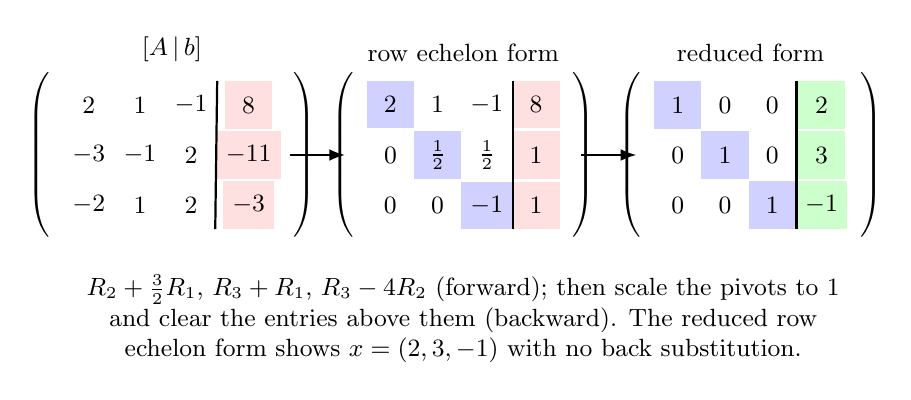
\begin{tikzpicture}[every node/.style={font=\small}, >={Latex[length=2mm]}]
	\matrix (A) [matrix of math nodes, nodes={minimum size=6mm, anchor=center}, left delimiter=(, right delimiter=), column sep=0pt, row sep=1pt] at (0,0) {
		2 & 1 & -1 & |[fill=red!12]| 8 \\
		-3 & -1 & 2 & |[fill=red!12]| -11 \\
		-2 & 1 & 2 & |[fill=red!12]| -3 \\
	};
	\draw[thick] (A-1-3.north east) -- (A-3-3.south east);
	\draw[->, thick] (1.5,0) -- (2.2,0);
	\matrix (B) [matrix of math nodes, nodes={minimum size=6mm, anchor=center}, left delimiter=(, right delimiter=), column sep=0pt, row sep=1pt] at (3.7,0) {
		|[fill=blue!18]| 2 & 1 & -1 & |[fill=red!12]| 8 \\
		0 & |[fill=blue!18]| \tfrac12 & \tfrac12 & |[fill=red!12]| 1 \\
		0 & 0 & |[fill=blue!18]| -1 & |[fill=red!12]| 1 \\
	};
	\draw[thick] (B-1-3.north east) -- (B-3-3.south east);
	\draw[->, thick] (5.2,0) -- (5.9,0);
	\matrix (C) [matrix of math nodes, nodes={minimum size=6mm, anchor=center}, left delimiter=(, right delimiter=), column sep=0pt, row sep=1pt] at (7.35,0) {
		|[fill=blue!18]| 1 & 0 & 0 & |[fill=green!20]| 2 \\
		0 & |[fill=blue!18]| 1 & 0 & |[fill=green!20]| 3 \\
		0 & 0 & |[fill=blue!18]| 1 & |[fill=green!20]| -1 \\
	};
	\draw[thick] (C-1-3.north east) -- (C-3-3.south east);
	\node[anchor=south] at (A.north) {$[A\,|\,b]$};
	\node[anchor=south] at (B.north) {row echelon form};
	\node[anchor=south] at (C.north) {reduced form};
	\node[anchor=north, align=flush center, text width=10cm] at (3.7,-1.4) {$R_2+\tfrac32R_1$, $R_3+R_1$, $R_3-4R_2$ (forward); then scale the pivots to $1$ and clear the entries above them (backward). The reduced row echelon form shows $x=(2,3,-1)$ with no back substitution.};
\end{tikzpicture}
\end{document}
